\documentclass[11pt,a4paper]{report} 
% Alternativ für doppelseitigen Ausdruck (nur bei > 60 Seiten sinnvoll)
% \documentclass[11pt,a4paper,twoside,openright]{report} 

% Deutsch
%\usepackage[german]{babel} % deutsch und deutsche Rechtschreibung
%\usepackage[english]{babel}
\usepackage[main=english, german]{babel}
\usepackage[utf8]{inputenc} % Unicode Text 
\usepackage[T1]{fontenc} % Umlaute und deutsches Trennen
\usepackage{textcomp} % Euro
\usepackage[hyphens]{url}
% statt immer Ab\-schluss\-ar\-beit zu schreiben
% einfach hier sammeln mit -. 
\hyphenation{Ab-schluss-ar-beit}
% Vorsicht bei Umlauten und Bindestrichen
\hyphenation{Ver-st\"ar-ker-aus-gang}
 % eigene Hyphenations, die für das Dokument gelten
\usepackage{amssymb} % Symbole
\usepackage{emptypage} % Wirklich leer bei leeren Seiten


%% Fonts, ein kompletter Satz an Optionen

% Times New Roman, gewohnter Font, ok tt und serifenlos
%\usepackage{mathptmx} 
%\usepackage[scaled=.95]{helvet}
%\usepackage{courier}

% Palatino mit guten Fonts für tt und serifenlos
\usepackage{mathpazo} % Palatino, mal was anderes
\usepackage[scaled=.95]{helvet}
\usepackage{courier}

% New Century Schoolbook sieht auch nett aus (macht auch tt und serifenlos)
%\usepackage{newcent}

% Oder default serifenlos mit Helvetica 
% ich kann es nicht mehr sehen ...
%\renewcommand{\familydefault}{\sfdefault}

\usepackage{microtype}

% Bilder und Listings
\usepackage{graphicx} % wir wollen Bilder einfügen
\usepackage{subfig} % Teilbilder
\usepackage{wrapfig} % vielleicht doch besser vermeiden
\usepackage{listings} % schöne Quellcode-Listings
% ein paar Einstellungen für akzeptable Listings
\lstset{basicstyle=\ttfamily, columns=[l]flexible, mathescape=true, showstringspaces=false, numbers=left, numberstyle=\tiny}
\lstset{language=python} % und nur schöne Programmiersprachen ;-)
% und eine eigene Umgebung für Listings
\usepackage{float}
\newfloat{listing}{htbp}{scl}[chapter]
\floatname{listing}{Listing}

% Seitenlayout
\usepackage[paper=a4paper,width=14cm,left=35mm,height=22cm]{geometry}
\usepackage{setspace}
\linespread{1.15}
\setlength{\parskip}{0.5em}
\setlength{\parindent}{0em} % im Deutschen Einrückung nicht üblich, leider

% Seitenmarkierungen 
\newcommand{\phv}{\fontfamily{phv}\fontseries{m}\fontsize{9}{11}\selectfont}
\usepackage{fancyhdr} % Schickere Header und Footer
\pagestyle{fancy}
\renewcommand{\chaptermark}[1]{\markboth{#1}{}}
%\fancyhead[L]{\phv \leftmark}
\fancyhead[L]{\phv \nouppercase{\leftmark}}
\fancyhead[R]{\phv \thepage}
% Unten besser auf alles Verzichten
%\fancyfoot[L]{\textsf{\small \kurztitel}}
\fancyfoot[C]{\ } % keine Seitenzahl unten
%\fancyfoot[R]{\textsf{\small Medieninformatik}}

% Theorem-Umgebungen
\newtheorem{definition}{Definition}[chapter]
\newtheorem{satz}{Satz}[chapter]
\newtheorem{lemma}[satz]{Lemma} % gleicher Zähler wie Satz
\newtheorem{theorem}{Theorem}[chapter]
\newenvironment{beweis}[1][Beweis]{\begin{trivlist}
\item[\hskip \labelsep {\textit{#1 }}]}{\end{trivlist}}
\newcommand{\qed}{\hfill \ensuremath{\square}}

% Quellen teilen
\usepackage{bibtopic} 

% Hochschule Logo, noch nicht perfekt
\usepackage{hsrmlogo}

% Spezialpakete
\usepackage{epigraph}
\setlength{\epigraphrule}{0pt} % kein Trennstrich

% damit wir nicht so viel tippen müssen, nur für Demo 
\usepackage{blindtext} 

% Zum Zeigen von Fehlern
\usepackage{soul}
\newcommand*\falsch{\st}

 % alle Pakete und Einstellungen

% Hier anpassen 
\newcommand{\welchethesis}{Bachelor}
% \newcommand{\welchethesis}{Master}
\newcommand{\thesisofwas}{of Science - B.Sc.}
\newcommand{\titel}{Study and implementation of a decentralized application that can provide
	permissionless financial services using an evm based blockchain}
%\newcommand{\kurztitel}{Template Abschlussarbeit}
\newcommand{\autor}{Mario Alberto Maita Orozco}
\newcommand{\datum}{30.06.2022} % Abgabedatum
\newcommand{\ort}{Wiesbaden}
\newcommand{\referent}{Prof.\ Dr.\ Eva-Maria Iwer}
\newcommand{\korreferent}{Prof.\ Dr.\ Marc-Alexander Zschiegner}

\usepackage{hyperref}
\hypersetup{
	colorlinks=true,
	linkcolor=blue,
	filecolor=magenta,      
	urlcolor=cyan,
	citecolor=blue,
%	pdftitle={Overleaf Example},
%	pdfpagemode=FullScreen,
}
\begin{document}

\begin{titlepage}
  \begin{center}
    % Kopf der Seite
    \hsrmlogo[1]
    \parbox[b]{8cm}{Hochschule RheinMain \\
     Fachbereich Design Informatik Medien \\
     Studiengang Informatik - Technische Systeme}
    \vfill    
    {\LARGE Bachelor-Arbeit} \\[0.5cm]
    {\large zur Erlangung des akademischen Grades} \\[5mm]
    {\large \welchethesis\ \thesisofwas} \\[5mm]
    \rule{\textwidth}{1pt}\\[0.5cm]
    {\begin{spacing}{1.15} \LARGE \bfseries \titel \\ \end{spacing}}
    \rule{\textwidth}{1pt}    
    \vfill    
    \begin{tabular}{ll} % Mitte der Seite
      Vorgelegt von & \autor \\
      am & \datum \\
      Referent & \referent \\
      Korreferent & \korreferent
    \end{tabular}    
    \vfill
  \end{center}
\end{titlepage}
\cleardoublepage


% Erklärung gemäß den Allgemeinen Bestimmungen für Prüfungsordnungen
% der Paragraph schwankt, daher ohne Nennung einer Nummer
\thispagestyle{empty}
\section*{Erklärung gem. ABPO, Ziff. 4.1.5.4}
Ich versichere, dass ich die Bachelor-Arbeit selbständig verfasst und keine anderen als
die angegebenen Hilfsmittel benutzt habe.
´

\vspace{6em}
\noindent\begin{tabular}{p{0.37\textwidth}p{0.56\textwidth}}
\ort, \datum  & \rule{0.56\textwidth}{0.5pt}\\
              & \makebox[1cm]{\ } \autor
\end{tabular}

\vfill

\section*{Erklärung zur Verwendung der \welchethesis thesis}

Hiermit erkläre ich mein Einverständnis mit den im Folgenden aufgeführten
Verbreitungsformen dieser Bachelor-Arbeit:

\vspace{1em}
\noindent\begin{tabular}{|p{0.82\textwidth}|c|c|}
  \hline
  \textbf{Verbreitungsform} & \makebox[0.035\textwidth]{\textbf{Ja}} 
                            & \makebox[0.05\textwidth]{\textbf{Nein}} \\\hline
  Einstellung der Arbeit in die Hochschulbibliothek 
                         mit Datenträger   &  & $\times$ \\\hline
  Einstellung der Arbeit in die Hochschulbibliothek  
                         ohne Datenträger  & $\times$ & \\\hline
  Veröffentlichung des Titels der Arbeit im Internet  
                                           & $\times$ & \\\hline
  Veröffentlichung der Arbeit im Internet             
                                           &  $\times$  & \\\hline
\end{tabular}

\vspace{6em}
\noindent\begin{tabular}{p{0.37\textwidth}p{0.56\textwidth}}
\ort, \datum  & \rule{0.56\textwidth}{0.5pt}\\
              & \makebox[1cm]{\ } \autor
\end{tabular}
\cleardoublepage

 % Titelseite, Erklärungen, etc.

\begin{abstract} 
abstract
\end{abstract}

\tableofcontents
\newpage 

\chapter{Introduction} \label{ch:intro}
%\epigraphhead[70]{\epigraph{Documentation is like sex: 
%when it is good, it is very, very good; and when it is bad, 
%sit is better than nothing.}{\textit{Dick Brandon}}}



\section{Motivation}
In the last years' blockchain technology has gained a lot of traction and many developers are willing to build applications on top of this technology.
The Ethereum network with the Ethereum Virtual Machine, or EVM~\ref{sec:evm}, (whose state is validated and copied by every node of the network) offers a new way of application development. Meaning that developers can now implement some functionality and deploy it to a public EVM blockchain, making the code/functionality tamper-resistant; in addition, the implemented functionality (or smart contract) can be called by any participant or other code/contracts within the network. This composability allows anyone to interact with already deployed contracts and build other applications on top of them. 
These kinds of applications are called Decentralized applications or Dapps~\ref{sec:dapps}, because they are built on top of a decentralized network such as  Ethereum.
\section{Goals}
The goals of this Thesis are, to study and provide a better understanding of: 
\begin{itemize}
	\item How Dapps are built.
	\item Which technology is used.
	\item And the development of a Dapp that uses well-known DeFi protocols see~\ref{ch:defi}, to let users access to permissionless financial services such as lending and borrowing of crypto assets.
\end{itemize}


\section{Thesis Structure}
The Thesis is divided into the following chapters:
\begin{itemize}
	
	\item \textbf{Chapter ~\ref{ch:background} - Fundamentals}, gives a technical overwiev of the blockchain technology and the Ethereum network.
	\item \textbf{Chapter ~\ref{ch:defi}} ...
	\item \textbf{Chapter ~\ref{ch:appreq}} ...
	\item \textbf{Chapter ~\ref{ch:impl}} ...
	\item \textbf{Chapter ~\ref{ch:conclusion}} ...
\end{itemize}


%%%%%
%%%%% Chapter
\chapter{Fundamentals} \label{ch:background}

\section{Blockchain} \label{sec:bc}
A blockchain\cite{book:bc}\cite{article:bc} is a type of database (append-only data strucuture), which stores data in blocks. These blocks are chronologically ordered by discrete timestamps and linked to each other using cryptographic hash functions\cite{chf}\cite{book:chf}. Commonly, a blockchain is used as a public distributed ledger of transactions records, shared and synchronized by a per-to-per network, where every party can participate in the validation of new blocks based on a consensus protocol, see~\ref{sec:cp}.
The idea of a cryptographically secured chain of blocks was originally presented by Haber and Stornetta\cite{time-stamp} in 1991. However, the implementation and adoption of this technology started with the conception of the bitcoin cryptocurrency whitepaper\cite{bitcoin} in 2008.

\begin{figure}[htp]
	\centering
	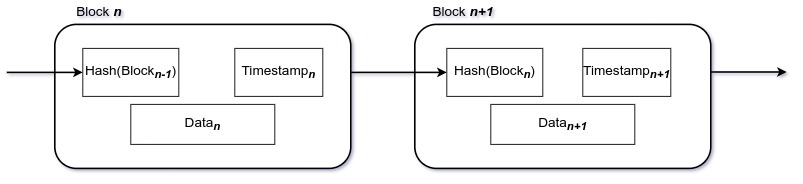
\includegraphics[width=0.9\textwidth]{./images/blockchain}
	\caption{View of two blocks in a blockchain}
	\label{fig:bc}
\end{figure}

Determined by the blockchain implementation, block contents can be different. A block usually has a timestamp, the data or transactions record, and the hash value of the previous block in the chain, see figure~\ref{fig:bc}.
The way that a blockchain ensures the security and keeps the integrity of the data is through cryptographic hash functions \ref{sec:chf}, and Merkle trees \ref{sec:mt}

By adding the cryptographic hash value of the previous block  (Block $n$ to Block $n+1$), blockchains ensure the integrity of previous blocks. Because of the second preimage resistance of cryptographic hash functions, see~\ref{sec:chf}, it is computationally infeasible to  find an input other then Block $n$ in order to generate an output = Hash (Block $n$). Due to that, the further the blockchain grows beyond block $n$, the more secure is the integrity of block $n$ and previous blocks.

Depending on who can participate in the consensus protocol, blockchain networks can be divided into two groups: permissionless and permissioned blockchains. This Thesis will be focused on permissionless blockchains that use an EVM, such as the Ethereum network.



\subsection{Cryptographic hash functions}\label{sec:chf}
A cryptographic hash function\cite{chf}\cite{book:chf} maps a given data of variable size to a fixed length \emph{n}-bit string called hash value. $ H : \{0,1\}^* \to \{0,1\}^n $ Such hash functions have the following properties:
\begin{enumerate}
		
	\item \textbf{Collision resistance}: Given $x_1, x_2 $ It should be necessary $ O(2^\frac{n}{2}) $ compute power such that $H(x_1) = H(x_2)$
	
	\item \textbf{Preimage resistance}: For a hash value \emph{h}, it should be necessary $ O(2^n) $ computation power in order to obtain an \emph{x} such that $ H(x)=h $.~~In other words, it should be a one-way function.
	
	\item \textbf{Second preimage resistance}: For an input $x_1$ and its hash value $h_1$, it should be necessary $ O(2^n) $ computation power in order to obtain a $x_2$ such that $H(x_2)=h_1$

	
\end{enumerate}

Such properties prevent attackers from modifying existing blocks keeping the blockchain intact. For example, the bitcoin network uses the SHA-256 hashing algorithm to validate a block, and append it to the chain. This means once a consensus among all the participants is done, and a new block is added, it will be required $ O(2^{256}) $ computation power to tamper with the blockchain. In other words, it is nearly impossible to manipulate an added block as a result of the tremendous computer power that would be needed.

\subsection{Merkle tree}\label{sec:mt}
A Merkle tree\cite{article:merkle}\cite{book:merkle} or hash tree is a binary tree where every leaf node (nodes at the bottom of the tree) is the cryptographic hash value of some data or transaction. A merkle tree is constructed bottom-up; the upwards nodes are the cryptographic hash values of its two child nodes. Therefore, the root node  will contain a complete fingerprint of the entire set of transactions. 

Merkle trees allow secure and efficient data verification using cryptographic hash functions. For example; if a participant in the network needs to verify the validity of these four transactions, see figure~\ref{fig:merkle}, only a check of the root hash value is necessary. Due to the Merkle tree structure, if any of the data blocks is modified, so will be the root hash value. Furthermore, Merkle tree is a very efficient data structure; for instance, checking that a given transaction is included in the tree will take a maximum of $2log (N)$ operations.
\begin{figure}[htp]
	\centering
	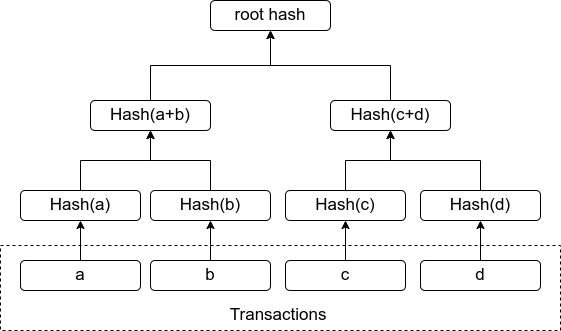
\includegraphics[width=0.7\textwidth]{./images/merkle}
	\caption{Merkle tree of four transactions}
	\label{fig:merkle}
\end{figure}
\subsection{Consensus Protocol}\label{sec:cp}
The consensus protocol\cite{article:bc} of a blockchain network gives a specific rule for verifying whether a transaction is valid or not. As mentioned in~\ref{sec:bc}, any participant or node of the network, depending on the blockchain type, can append a new block. For the reason that blockchains typically do not have a centralized authority validating transactions, participants on the blockchain must verify any transaction according to the set of rules or consensus protocol of the blockchain. The most common consensus mechanisms nowadays are:
\begin{itemize}
	\item[] \textbf{Proof of work (PoW)}
	In a PoW blockchain, nodes have to solve a cryptographic task in order to validate a block, the first node to find a solution can submit the transaction. Most of the first blockchains in the space use proof-of-work-based protocols; for example, Bitcoin uses PoW based on the cryptographic hash function SHA-256.	
	\item[] \textbf{Proof of state (PoS)}
	In a PoS blockchain, the entity that can validate a transaction is randomly selected, depending on the "stake" that a node has on the network. Since nodes have a large stake in the blockchain, they will pursue the integrity of the network.

\end{itemize}
\subsection{Public-Key Cryptography}
In order to interact with a blockchain, participants use public key cryptography or asymmetric key cryptography\cite{book:pkc}. The public key acts as the id of the sender or receiver of a given message; and it can be shared with others without any security downfall. On the other hand, the private key should be kept secure and private by the message sender; it is used to sign (digital signature) the messages or transactions, i.e., give permission to change the state of the user records in the blockchain.

\textbf{Digital signature:} The message or transaction can only be signed with a private key, and anyone who knows the public key of the signed message can verify  its authenticity. Meaning that any party of the blockchain can participate in the verification of the transactions/messages.

The private key is a random number and the public key is generated from it using one-way cryptographic hash functions, see \ref{sec:chf} or elliptic curve cryptography\cite{book:pkc}\cite{wiki:ecc}. Elliptic curve cryptography (ECC) is based on the discrete logarithm problem and is the most common public-key algorithm in blockchain networks.
In mathematics terms, an elliptic curve is a plane curve over all the points $(x, y)$ that satisfy the following equation:  $ y^2 = x^3 +ax + b $

%\subsection{Bitcoin}
%The bitcoin network is a set of technologies that enabled for the first time a %decentralized, permissionless, trustless, peer-to-peer digital currency system. %The distributed computation system that bitcoin introduced: the proof-of-work %algorithm to produce a consensus in a distributed system without a central %trusted authority, in combination with the blockchain storage system, solved the %double-spend problem and the Byzantine generals problem.

\section{Ethereum}
The Bitcoin\cite{bitcoin}\cite{book:masteringBTC} network and its set of technologies enabled for the first time a decentralized, permissionless, trustless, peer-to-peer digital currency system. The distributed computation system that bitcoin introduced: a proof-of-work algorithm to produce a consensus in a distributed system without a central trusted authority, in combination with the blockchain storage system, solved the double-spend problem and the Byzantine generals problem, enabling other applicability beyond digital currencies.  In 2014, Vitalik Butering introduced Ethereum\cite{article:eth}, a platform that moved beyond cryptocurrency applications.

Similar to Bitcoin, Ethereum\cite{article:eth}\cite{book:masteringETH} is a distributed transaction-based state machine. However, it is not only a cryptocurrency system. Ethereum is a decentralized computing platform or a decentralized, pseudo-turning complete virtual machine, which runs smart contracts and stores its state changes in its blockchain. Like bitcoin, state changes in ethereum are managed by a consensus mechanism, where everyone can participate in the validation of  blocks or state changes.

\subsection{Accounts}
Ethereum\cite{article:eth}\cite{wood2014ethereum} has an account-based model, where every account represents a state. An account is mapped with a 160 bits address (public key) and there are two types of accounts: Externally owned account (EOA), controlled by a private key and contract account, controlled by EVM code. Depending on the account type, an account state is represented by the following four fields: \textbf{Nonce} is a counter that represents the number of transactions or contracts created by the account. \textbf{Balance} is the amount of Ether owned by the account, expressed in Wei. \textbf{Storage hash} is the root hash of a merkle tree that represents the contents of the account. \textbf{Code hash} is the hash that points to the EVM code that the account has.
\begin{figure}[htp]
	\centering
	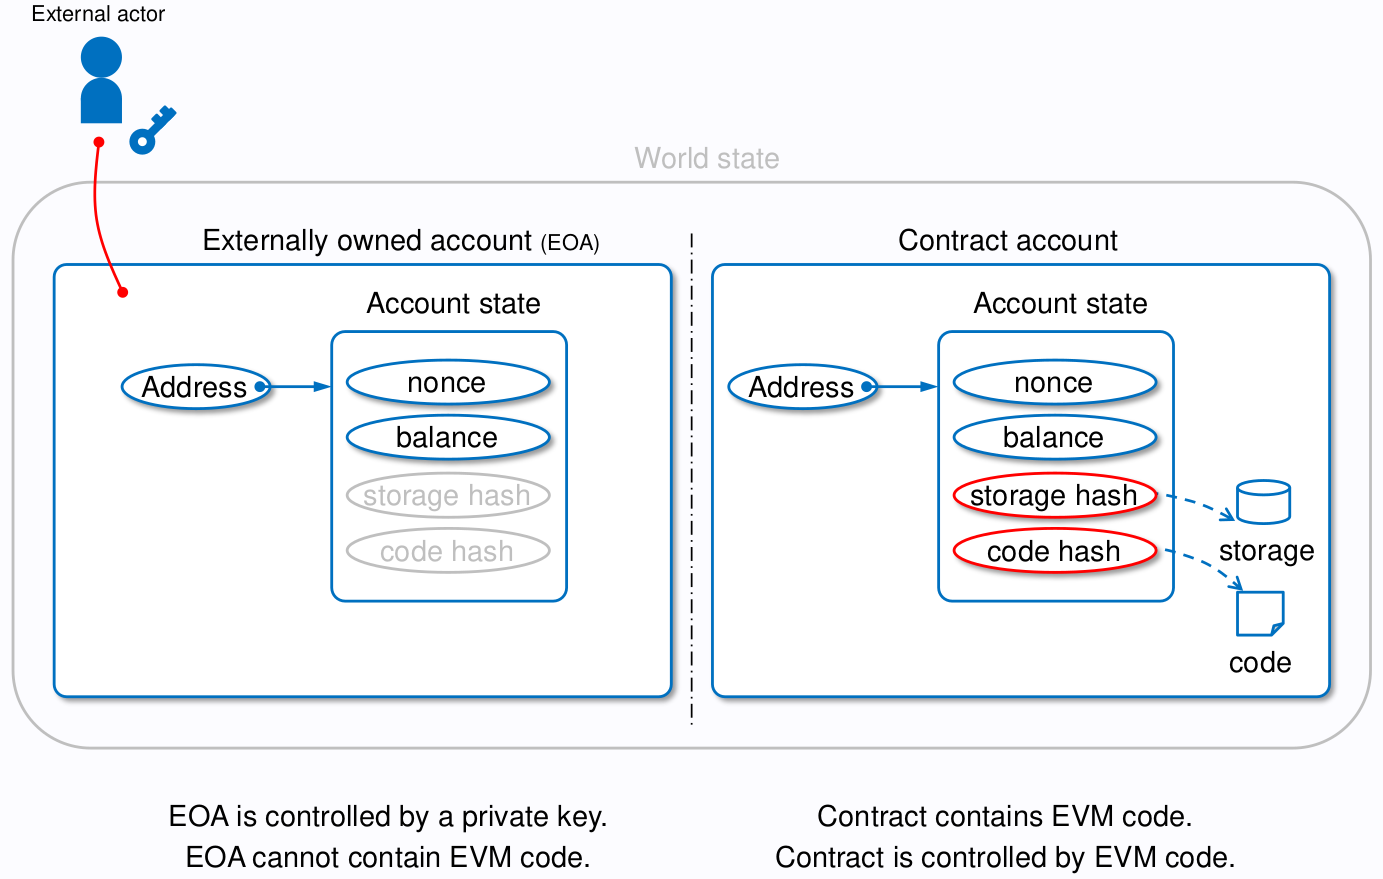
\includegraphics[width=0.8\textwidth]{./images/accounts}
	\caption{Ethereum Accounts\cite{evm-illustrate}}
	\label{fig:accounts}
\end{figure}

\subsubsection{Transactions and Messages}
A \textbf{transaction} is a cryptographically-signed message that can only be sent by an EOA. Transactions can trigger a state change on the blockchain or the execution of EVM code. Transactions can be divided into two groups:
\begin{itemize}
	\item  \textbf{Message calls}: The transactions between accounts.
	\item \textbf{Contract creations}: creation of a new account with EVM code in its data field.
\end{itemize}
\textbf{Messages} can be seen as internal transactions between contracts triggered by a message call. A message is like a transaction but produced by a contract. This way messages enable contracts to interact between them.
\subsection{Ethereum Virtual Machine (EVM)}\label{sec:evm}
\subsection{Smart Contracts}\label{sec:sc}
\subsection{Solidity}\label{sec:sol}
\subsection{Tokens}\label{sec:tokens}
\subsection{Decentralized Applications (Dapps)}\label{sec:dapps}

%%%%%%%%%%%% FIGURE
%\begin{figure}[htp]
%\centering
%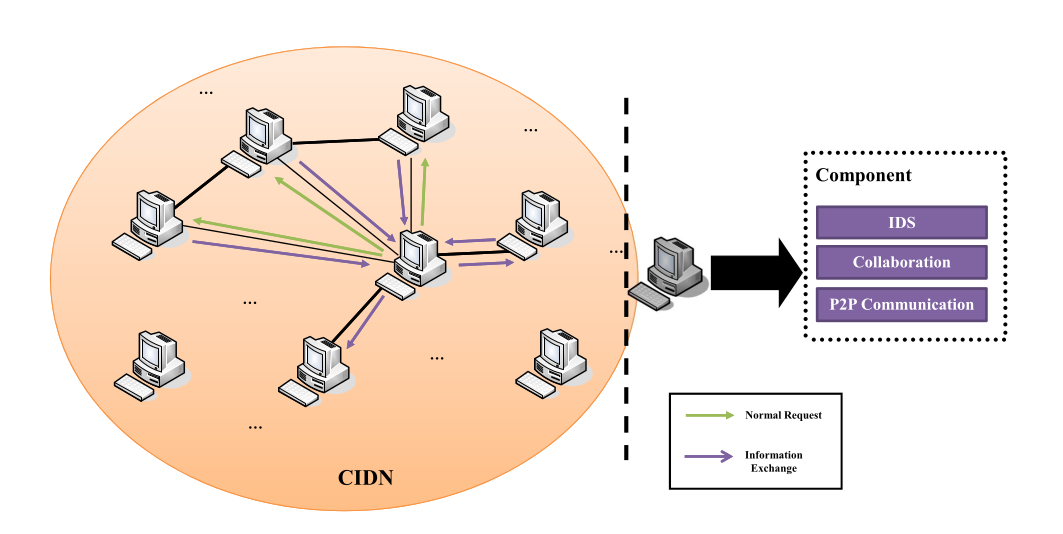
\includegraphics[width=.9\textwidth]{images/cids}
%\caption{Dateien zur Erstellung des Templates}
%\label{fig:templateprozess}
%\end{figure}

%%%%%
%%%%% Chapter
\chapter{Decentralized Finance (DeFi)} \label{ch:defi}

%%%%%
%%%%% Chapter
\chapter{Application requirements} \label{ch:appreq}

%\section{Listings} \label{sec:listings}
%\begin{listing}[htbp]
%\begin{lstlisting}
%def ggt(x, y):
%    while x != 0:
%        x,y = y%x, x
%    return y
%\end{lstlisting}
%\caption{ggT --- kurz und gut}
%\label{code:ggt}
%\end{listing}


%%%%%
%%%%% Chapter
\chapter{Implementation and testing} \label{ch:impl}
\newpage


%%%%%
%%%%% Chapter
\chapter{Conclusion and future work} \label{ch:conclusion}

\newpage

% Listen wenn überhaupt ans Ende und nicht an den Anfang.
% Meist ist das aber unnötig.
%\listoffigures % Liste der Abbildungen 
%\listoftables % Liste der Tabellen
% \newpage

\bibliographystyle{plain} % Literaturverzeichnis
\begin{btSect}{thesis} % mit bibtopic Quellen trennen
\section*{Bibliography}
\btPrintCited
\end{btSect}
\begin{btSect}{online}
\section*{Online Sources}
\btPrintCited
\end{btSect}
% dann mit "bibtex thesis1" und "bibtex thesis2" arbeiten

\end{document}
;;; Local Variables:
;;; ispell-local-dictionary: "de_DE-neu"
;;; End:
